\documentclass[twoside]{article}
\setlength{\oddsidemargin}{0.25 in}
\setlength{\evensidemargin}{-0.25 in}
\setlength{\topmargin}{-0.6 in}
\setlength{\textwidth}{6.5 in}
\setlength{\textheight}{8.5 in}
\setlength{\headsep}{0.75 in}
\setlength{\parindent}{0 in}
\setlength{\parskip}{0.1 in}
\newcommand{\eqdef}{:\mathrel{\mathop=}}
\newcommand{\norm}[1]{\left\lVert #1 \right\rVert}

%
% ADD PACKAGES here:
%

\usepackage{amsmath,amsfonts,graphicx}

%
% The following commands set up the lecnum (lecture number)
% counter and make various numbering schemes work relative
% to the lecture number.
%
\newcounter{lecnum}
\renewcommand{\thepage}{\thelecnum-\arabic{page}}
\renewcommand{\thesection}{\thelecnum.\arabic{section}}
\renewcommand{\theequation}{\thelecnum.\arabic{equation}}
\renewcommand{\thefigure}{\thelecnum.\arabic{figure}}
\renewcommand{\thetable}{\thelecnum.\arabic{table}}

%
% The following macro is used to generate the header.
%
\newcommand{\lecture}[4]{
   \pagestyle{myheadings}
   \thispagestyle{plain}
   \newpage
   \setcounter{lecnum}{#1}
   \setcounter{page}{1}
   \noindent
   \begin{center}
   \framebox{
      \vbox{\vspace{2mm}
    \hbox to 6.28in { {\bf Advanced Machine Learning
	\hfill Fall 2020} }
       \vspace{4mm}
       \hbox to 6.28in { {\Large \hfill Lecture #1: #2  \hfill} }
       \vspace{2mm}
       \hbox to 6.28in { {\it  #3 \hfill  #4} }
      \vspace{2mm}}
   }
   \end{center}
   \markboth{Lecture #1: #2}{Lecture #1: #2}

   {\bf Note}: {\it LaTeX template courtesy of UC Berkeley EECS dept.}

   {\bf Disclaimer}: {\it These notes are adapted from CMU's 10-725 Course, Stanford's CS229 Course, ETH's Advanced Machine Learning Course and  Bishop's "Pattern Recognition and Machine Learning" book.}
   \vspace*{4mm}
}
%
% Convention for citations is authors' initials followed by the year.
% For example, to cite a paper by Leighton and Maggs you would type
% \cite{LM89}, and to cite a paper by Strassen you would type \cite{S69}.
% (To avoid bibliography problems, for now we redefine the \cite command.)
% Also commands that create a suitable format for the reference list.
\renewcommand{\cite}[1]{[#1]}
\def\beginrefs{\begin{list}%
        {[\arabic{equation}]}{\usecounter{equation}
         \setlength{\leftmargin}{2.0truecm}\setlength{\labelsep}{0.4truecm}%
         \setlength{\labelwidth}{1.6truecm}}}
\def\endrefs{\end{list}}
\def\bibentry#1{\item[\hbox{[#1]}]}

%Use this command for a figure; it puts a figure in wherever you want it.
%usage: \fig{NUMBER}{SPACE-IN-INCHES}{CAPTION}
\newcommand{\fig}[3]{
			\vspace{#2}
			\begin{center}
			Figure \thelecnum.#1:~#3
			\end{center}
	}
% Use these for theorems, lemmas, proofs, etc.
\newtheorem{theorem}{Theorem}[lecnum]
\newtheorem{lemma}[theorem]{Lemma}
\newtheorem{proposition}[theorem]{Proposition}
\newtheorem{claim}[theorem]{Claim}
\newtheorem{corollary}[theorem]{Corollary}
\newtheorem{definition}[theorem]{Definition}
\newenvironment{proof}{{\bf Proof:}}{\hfill\rule{2mm}{2mm}}

% **** IF YOU WANT TO DEFINE ADDITIONAL MACROS FOR YOURSELF, PUT THEM HERE:

\newcommand\E{\mathbb{E}}

\begin{document}
%FILL IN THE RIGHT INFO.
%\lecture{**LECTURE-NUMBER**}{**DATE**}{**LECTURER**}{**SCRIBE**}
\lecture{7}{Support Vector Machines}{}{}
%\footnotetext{These notes are partially based on those of Nigel Mansell.}

% **** YOUR NOTES GO HERE:

% Some general latex examples and examples making use of the
% macros follow.  
%**** IN GENERAL, BE BRIEF. LONG SCRIBE NOTES, NO MATTER HOW WELL WRITTEN,
%**** ARE NEVER READ BY ANYBODY.


\section{Lagrangian} % Don't be this informal in your notes!

Consider a general minimization problem. There is no need for it to be convex, let's keep it as general as possible.

\begin{equation*}
\begin{aligned}
& \underset{x}{\text{minimize}}
& & f(x) \\
& \text{subject to}
& & h_i(x) \leq 0, \; i = 1, \ldots, m \\
&&& l_j(x)\equiv 0, \; j = 1, \ldots, r
\end{aligned}
\end{equation*}
\\

The Lagrangian is defined as:
\begin{equation}
    \mathcal{L}(x,u,v) = f(x) +  \sum_{i=1}^{m} u_i \cdot h_i(x) + \sum_{j=1}^{r} v_j \cdot l_j(x)
\end{equation}


Where $u \in {\mathbb{R}^m \geq 0}$, $v \in {\mathbb{R}^r}$.
\\
\\
(Small side-note) We define the Lagrangian $\mathcal{L}(x,u,v) = - \infty$ for values of  $u < 0$.\\
\\ We are going to exploit the following property of the Lagrangian: \\
$\forall u \geq 0$ and $\forall v$ :
\textbf{$f(x) \geq \mathcal{L}(x,u,v) $ at each feasible $x$}


\begin{figure}[h]
\caption{Each dotted line shows $\mathcal{L}(x, u)$ for different choice of $u \geq 0$.}
\centering
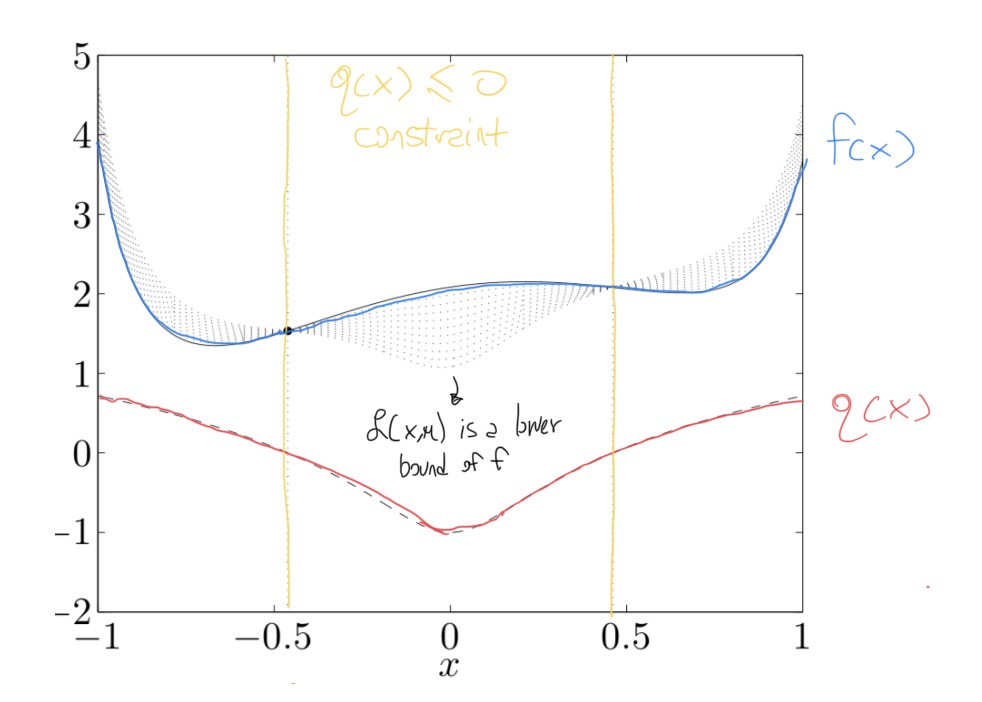
\includegraphics[width=0.39\textwidth]{img/lagrangian.jpg}
\end{figure}





\newpage




\subsection{Lagrangian Dual Function}
Let $C$ denote the primal feasible set, $f^{*}$ denote primal optimal value. Minimizing $\mathcal{L}(x, u, v)$ over all $x$ gives a
lower bound:

\begin{equation*}
\begin{aligned}
f^{*} \overset{(i)}{\geq} \underset{x \in {C}}{\text{min}}& & \mathcal{L}(x, u, v) \overset{(ii)}{\geq} \underset{x}{\text{min}}& & \mathcal{L}(x, u, v)  \eqdef g(u,v)
\end{aligned}
\end{equation*}
\\

Where $(i)$ derives from the property we stated earlier taking the minimum of both sides and $(ii)$ holds because the unconstrained minimum will always be less or equal the constrained one. \\

We call $g(u,v)$ the Lagrangian dual function and it gives a lower bound on $f^{*}$. The main takeaway here is that $(i)$ is often not computable because of the constraints. Hence, we prefer to solve the dual problem $(ii)$.

\subsection{Langrange Dual Problem}
Given a primal problem 

\begin{equation*}
\begin{aligned}
& \underset{x}{\text{minimize}}
& & f(x) \\
& \text{subject to}
& & h_i(x) \leq 0, \; i = 1, \ldots, m \\
&&& l_j(x)\equiv 0, \; j = 1, \ldots, r
\end{aligned}
\end{equation*}

We have showed that our dual function satisfies $f^{*}  \geq g(u,v)$ for all $u \geq 0$ and $v$ \\
Thus, we can get the best lower-bound estimate of $f^{*}$ maximizing $g(u,v)$ over the feasible $u,v$, yielding the Lagrange Dual Problem:

\begin{equation*}
\begin{aligned}
& \underset{u,v}{\text{max}}
& & g(u,v) \\
& \text{subject to}
& & u \geq 0, \;
\end{aligned}
\end{equation*}\\

 A key property is called \textbf{weak duality}: 
\begin{equation*}
    f^{*} \geq g^{*}
\end{equation*}
Where $f^{*},g{*}$ are the optimal values for the primal and dual problems.\\Note that this property always holds, even if the primal problem is not convex. Furthermore, it is easy to prove that  \textbf{the dual problems is always a convex optimization problem}, even if the primal problem is non convex.

\newpage
\subsection{Strong Duality}
In some problems we will have $f^{*}=g^{*}$, this property is called Strong Duality.

\begin{theorem}{(Slater's Condition)}
\\If the primal problem is a convex problem
and there exists at least one strictly feasible $x \in \mathbb{R} $, then Strong Duality holds.
\end{theorem}

In other words, the condition is that exists $x$ such that:

\begin{align*}
       h_i(x) < 0, \; i = 1, \ldots, m \\\\        
    l_j (x) = 0,\; j = 1, \ldots, r \\ 
\end{align*}



\subsection{Karush-Kuhn-Tucker (KKT) Conditions}

Given a general problem

\begin{equation*}
\begin{aligned}
& \underset{x}{\text{minimize}}
& & f(x) \\
& \text{subject to}
& & h_i(x) \leq 0, \; i = 1, \ldots, m \\
&&& l_j(x)\equiv 0, \; j = 1, \ldots, r
\end{aligned}
\end{equation*}

The KKT conditions are:
\begin{enumerate}
    \item $0 \in \partial_x (\mathcal{L}(x, u, v)  )$ (stationarity)
    \item $u_i \cdot h_i(x) = 0$ for all $i$ (complementary slackness)
    \item $h_i(x) \leq 0,  l_j(x)  = 0$ for all $i,j$ (primal feasibility)
    \item $u_i \geq 0$ for all $i$ (dual feasibility)
\end{enumerate}

\begin{theorem}
For $x^{*}$ and $u^{*}$, $v^{*}$ to be primal and dual solutions, KKT conditions are sufficient. 
\end{theorem}

\begin{proof}
$g^* = g(u^{*},v^{*}) = f(x^{*}) +  \sum_{i=1}^{m} u_i^{*} \cdot h_i(x^{*}) + \sum_{j=1}^{r} v_j^{*} \cdot l_j(x^{*})  = f(x^{*}) = f^* $ \\
\\ Where the first equality holds from stationarity and the second equality holds from complementary slackness and primal feasibility.
\end{proof}

\newpage 

\begin{theorem}
For a problem with strong duality (e.g. assume Slater's condition holds)\\
 $x^{*}$ and $u^{*}$, $v^{*}$ are primal and dual solution $\iff$ $x^{*}$ and $u^{*}$, $v^{*}$ satisfy KKT conditions.
\end{theorem}

\begin{proof}\\
\\
\textbf{Sufficiency:} Follows from Theorem 7.2.\\ \\ \textbf{Necessity:} Suppose $x^{*}$ and $u^{*}$, $v^{*}$ to be primal and dual solution, and suppose strong duality holds. Then:\\
\\ $f^* =g^* =  g(u^{*},v^{*}) $ \ (holds by assumptions)\\   
\\$=   \underset{x}{\text{min}}
& &( f(x) +  \sum_{i=1}^{m} u_i^{*} h_i(x) +\sum_{j=1}^{r} v_j^{*} \cdot l_j(x) ) $ \ (holds by definition)  \\ \\
$\leq   f(x^{*}) +  \sum_{i=1}^{m} u_i^{*} \cdot h_i(x^{*}) + \sum_{j=1}^{r} v_j^{*} \cdot l_j(x^{*})$ \ (min(f) is less or equals than the value of f at any other point) \\ \\
$\leq f(x^{*})$ \ (holds by feasibility since the sums must be less or equal than 0)  \\

The LHS equals RHS, therefore all the inequalities must be equalities. Looking at KKT Conditions:
\begin{itemize}
    \item \textbf{Primal and dual feasibility} hold by virtue of optimality: $x^*,u^*,v^*$ are optima $ \implies$ $x^*,u^*,v^*$ must be feasible
    \item \textbf{Stationarity} comes from the fact that $x^{*}$ minimizes $g(u^{*},v^{*})$. Since $x^{*}$ is the minimizer it must be a stationary point for this function.
    \item \textbf{Complementary Slackness} comes from the last inequality, since $\sum_{i=1}^{m} u_i^{*} \cdot h_i(x^{*})$ must  be equal to 0.
\end{itemize}


\end{proof}
\newpage

\section{Maximum Margin Classifiers}

We begin our discussion of Support Vector Machines by returning to the two-class classification problem using a linear model of the form:

\begin{equation*}
    y(x) = w^T  \phi(x) + b
\end{equation*}

We shall assume for the moment that the training data is linearly separable. The SVMs approach this problem through the concept of margin, which is defined to be the smallest distance between decision boundary and any of the samples. 

\subsection{Finding the margin}

Consider an arbitrary point $x$ and let $x_{\bot}$ be its orthogonal projection onto the decision surface, so that:

\begin{equation*}
    x = x_{\bot} + r  \dfrac{w}{\norm{w}}
\end{equation*}
    
Multiplying both sides of this result by $w^T$ and adding $b$ we get:
\begin{equation*}
    w^T  x + b = w^T  x_{\bot} + r w^T  \dfrac{w}{\norm{w}} + b
\end{equation*}

Applying the definition $y(x) = w^T  x + b$:
\begin{equation*}
    y(x) = y(x_{\bot}) + r  \norm{w}
\end{equation*}

From Figure 7.2 it is clear that $x_{\bot}$ lies on the decision surface, hence $y(x_{\bot})=0$. Solving for r:

\begin{equation*}
    r = \dfrac{y(x)}{\norm{w}}
\end{equation*}

Therefore, the perpendicular distance of a point $x$ from a hyperplane defined by $y(x)=0$ is given by:
\begin{equation*}
    \dfrac{\lvert y(x) \rvert}{\norm{w}}
\end{equation*}
\begin{figure}[h]
\caption{The decision surface shown in red is perpendicular to w.}
\centering
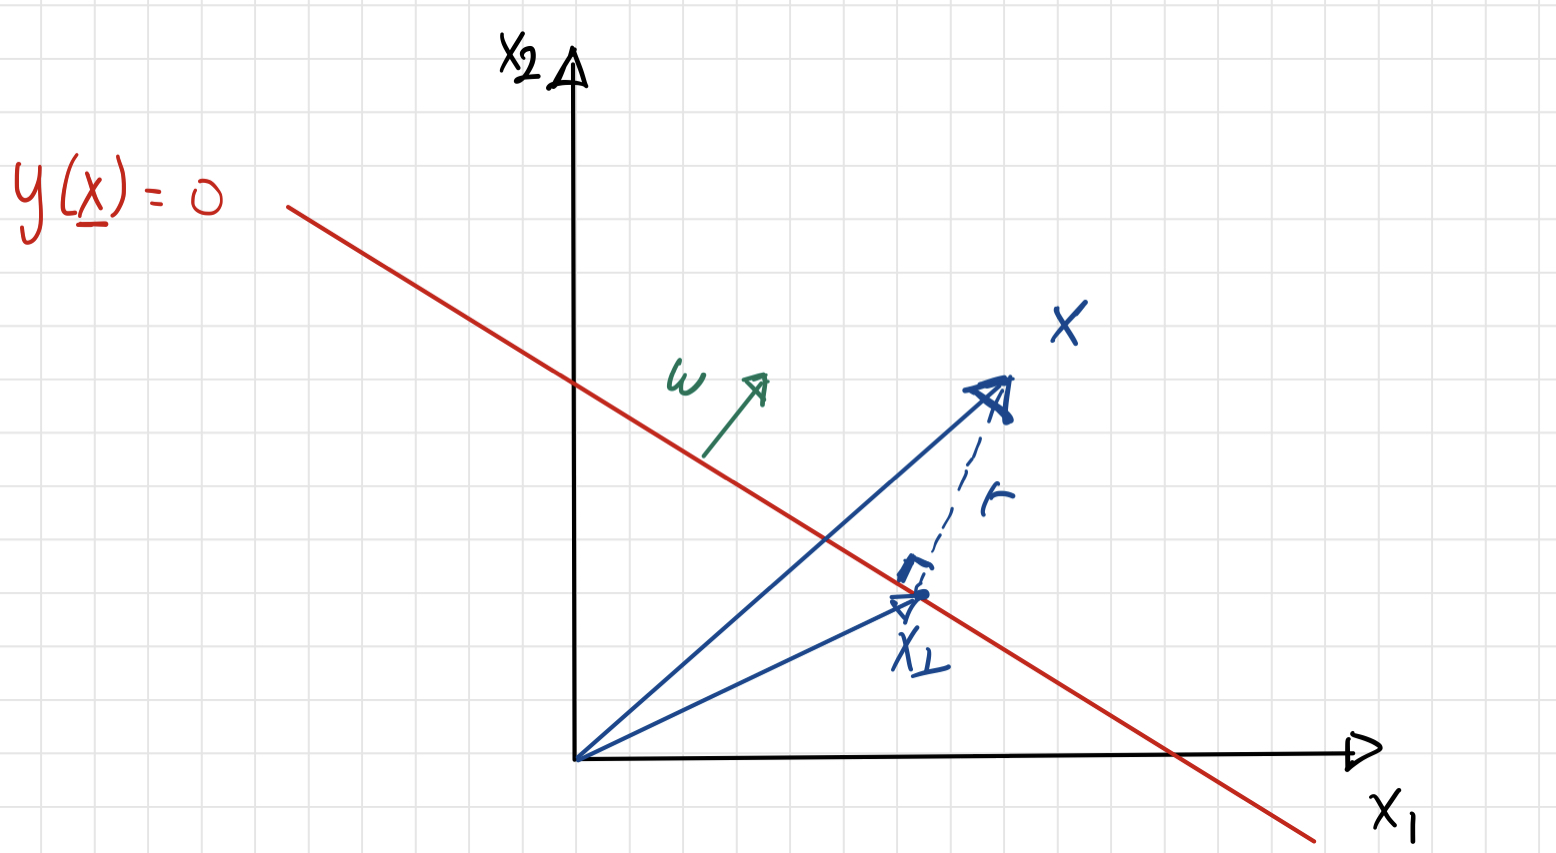
\includegraphics[width=0.385\textwidth]{img/margin.jpg}
\end{figure}

\newpage

\subsection{SVMs Primal Problem}

We wish to optimize the parameters $w$ and $b$ in order to maximize the minimum margin among all data points:

\begin{equation*}
\max_{w,b} \  \min_{n}   \dfrac{\lvert y(x_{n}) \rvert}{\norm{w}} 
\end{equation*}

We can take the factor $\dfrac{1}{\norm{w}}$ outside of the optimization over $n$ because it does not depend on $n$:

\begin{equation*}
\max_{w,b} \dfrac{1}{\norm{w}} \ \min_{n}  [t_{n} (w^T \phi(x) +b) ]
\end{equation*}

Direct solution of this optimization problem would be very complex (non-convex), and so we shall convert it into an equivalent problem that is much easier to solve. 

To do this, we note that if we make the rescaling $w' = kw$ and $b' = kb$ the margin will remain unchanged: 
\begin{equation*}
    r' = \dfrac{t_{n}((w')^T \phi(x_{n}) +b')}{\norm{w'}} = \dfrac{k t_{n} (w^T \phi(x_{n}) + b)}{k \norm{w}} = r
\end{equation*}

We can use this freedom to set the point that is closer to the decision surface:
\begin{equation*}
    t_{n} (w^T \phi(x_{n}) +b) = 1
\end{equation*}

In this case all data points will have to satisfy the constraints:

\begin{equation*}
    t_{i} (w^T \phi(x_{i}) +b) \geq 1 \ \ i = 1,\dotsc,N
\end{equation*}

Thus we can reduce the problem to:
\begin{equation*}
\begin{aligned}
& \underset{w,b}{\text{max}}
& & \dfrac{1}{\norm{w}}\\
& \text{subject to}
& & 1 - t_{i} (w^T \phi(x_{i}) +b)  \leq 0, \; i = 1, \ldots, N \\
\end{aligned}
\end{equation*}

Furthermore, maximizing ${\norm{w}^{-1}}$ is equivalent to minimizing $ \norm{w}^2$.We include a factor $1/2$ for later convenience:
\begin{equation*}
\begin{aligned}
& \underset{w,b}{\text{min}}
& & \dfrac{1}{2} \norm{w}^2\\
& \text{subject to}
& & 1 - t_{i} (w^T \phi(x_{i}) +b)  \leq 0, \; i = 1, \ldots, N \\
\end{aligned}
\end{equation*}

Two important observations:
\begin{itemize}
    \item It appears that the bias parameter b has disappeared from the optimization. However, it is determined implicitly via the constraints.
    \item The solution to a QP problem in $M$ variables has computational complexity that is $O(M^3)$. Thus, the primal problem is only feasible if we constrain ourselves to a fixed set of basis function (small $M$).  
\end{itemize}

\newpage

\subsection{SVMs Dual Problem}

First thing first, we should check if Slater's conditions is satisfied (remember that Slater's condition is sufficient for \textbf{strong duality}).\\
Let $w^*,b^*$ be an optimal solution and $\lambda > 1$, then $\lambda w^*, \lambda b^*$ will be strictly feasible:

\begin{equation*}
    t_{i}(\lambda w^{*T} \phi(x_{i}) + \lambda b^*) =  t_{i} \lambda ( w^{*T} \phi(x_{i}) +  b^*) > t_{i}  ( w^{*T} \phi(x_{i}) +  b^*) \geq 1, \; i = 1, \ldots, N \\
\end{equation*}

Since strong duality holds, we can solve the dual problem:

\begin{equation*}
\begin{aligned}
& \underset{a}{\text{max}}
&  \underset{w,b}{\text{min}}
& \ \mathcal{L}(w,b,a) \\
& \text{subject to}
& & a_{i} \geq 0, \; i = 1, \ldots, N \
\end{aligned}
\end{equation*}

Where we define the Lagrangian Dual Function $\mathcal{L}(w,b,a) = \dfrac{1}{2} \norm{w}^2 + \sum_{i=1}^{N} a_i\{ 1- t_{i}(w^T \phi(x_{i}) +b) \} $

Setting the derivatives of $\mathcal{L}(w,b,a)$ with respect to $w$ and $b$ equal to zero, we obtain the following two conditions:

\begin{align}
       w = \sum_{i=1}^{N} a_{i}t_{i}\phi(x_{i})  \\        
    \sum_{i=1}^{N} a_{i}t_{i} = 0
\end{align}


Now we substitute the conditions back into $\mathcal{L}(w,b,a)$:

\begin{equation*}
    \mathcal{L}(w,b,a) = \dfrac{1}{2} \norm{w}^2 + \sum_{i=1}^{N} a_{i} 
    - \overbrace{\sum_{i=1}^{N} a_{i}t_{i}b}^\text{=0} - \sum_{i=1}^{N} a_{i}t_{i} w^T \phi(x_{i})
\end{equation*}

Substituting (7.2) we obtain:

\begin{equation*}
    \mathcal{L}(a) = \dfrac{1}{2} \  [\sum_{i=1}^{N} a_{i}t_{i}\phi(x_{i})]^T [\sum_{i=1}^{N} a_{i}t_{i}\phi(x_{i})] + \sum_{i=1}^{N} a_{i} - \sum_{i=1}^{N} a_{i} t_{i} [\sum_{i=1}^{N} a_{i}t_{i}\phi(x_{i})]^T \phi(x_{i})
    \end{equation*}
    
Expanding the products:
\begin{equation*}
    \mathcal{L}(a) = \dfrac{1}{2} \  \sum_{i=1}^{N} { \sum_{j=1}^{N} a_{i} a_{j} t_{i} t_{j} \phi(x_{i})^T \phi(x_{j})}
    + \sum_{i=1}^{N} a_{i}  -
    \sum_{i=1}^{N} { \sum_{j=1}^{N} a_{i} a_{j} t_{i} t_{j} \phi(x_{i})^T \phi(x_{j})}
    \end{equation*}
\newpage
This gives the dual representation of the SVM problem:

\begin{equation*}
\begin{aligned}
& \underset{a}{\text{max}}
& & \sum_{i=1}^{N} a_{i}  - \dfrac{1}{2}
    \sum_{i=1}^{N} { \sum_{j=1}^{N} a_{i} a_{j} t_{i} t_{j} \phi(x_{i})^T \phi(x_{j})}\\
& \text{subject to}
& & a_{i}  \geq 0, \; i = 1, \ldots, N \\
&&& \sum_{i=1}^{N} a_{i}t_{i} = 0, 
\end{aligned}
\end{equation*}

Some important observations:
\begin{itemize}
    \item Note that now the time complexity for the QP solver is $O(N^3)$, thus it does not depend on the choice of basis function. For a fixed set of basis functions whose number M is smaller than the number N of data points, the dual problem appears disadvantageous. However, the dual problem makes feasible applying SVMs to feature spaces whose dimensionality exceed the number of data points, including infinite feature spaces. 
    \item In order to classify new data points using the trained model, we evaluate the sign of $y(x)$: 
    \begin{equation*}
        y(x) = \sum_{i=1}^{N}  a_{i}t_{i} \phi(x_i)^T \phi(x) +b
    \end{equation*}
    \item Remember that : Strong Duality  $\implies$ KKT conditions are satisfied. Hence, the following condition must hold:
    
    \begin{equation*}
         a_{i}(t_{i}y(x_{i})-1) = 0, \; i = 1, \ldots, N
    \end{equation*}
    
    Any data point for which $a_{i} = 0$ plays no role in making predictions for new data points. The remaining data points correspond to points that lie on the maximum margin hyperplanes in feature space and they are called support vectors. This property is central to the practical applicability of SVMs: once the model is trained, a significant proportion of the data points can be discarded.
    
\end{itemize}






\end{document}
